\section{Particle Physics detectors}

In order to detect a particle it must interact with the material of the detector and transfer energy in some recognisable fashion.
\paragraph{Particle detection occurs via the energy loss of particles through the material they traverse.} In the end, all signals we record are electromagnetic signals. So we can discover charged particles. Neutral particles need to be converted to charged particles to be seen. This happens in an electromagnetic calorimeter with photons $\gamma \to e^+ e^-$, and in hadronic calorimeters via nuclear interactions that create charged pions and protons.

\paragraph{Possibilities}
\begin{itemize}
\item[(i)] EM charged particles $\rightarrow$ Ionisation, Bremsstrahlung$^*$, Cherenkov
\item[(ii)] Hadrons $\rightarrow$ Nuclear interactions$^*$ (equivalent to ones above the involving the strong force)
\item[(iii)] Photons $\rightarrow$ Pair production$^{**}$, Photoelectric effect, Compton effect
\end{itemize}
$^{(*)}$ Cause a shower of particles (see later).\newline
$^{(**)}$ Total energy loss via a single interaction converting into charged particles.\newline
Some examples of what these processes look like:

\begin{center}
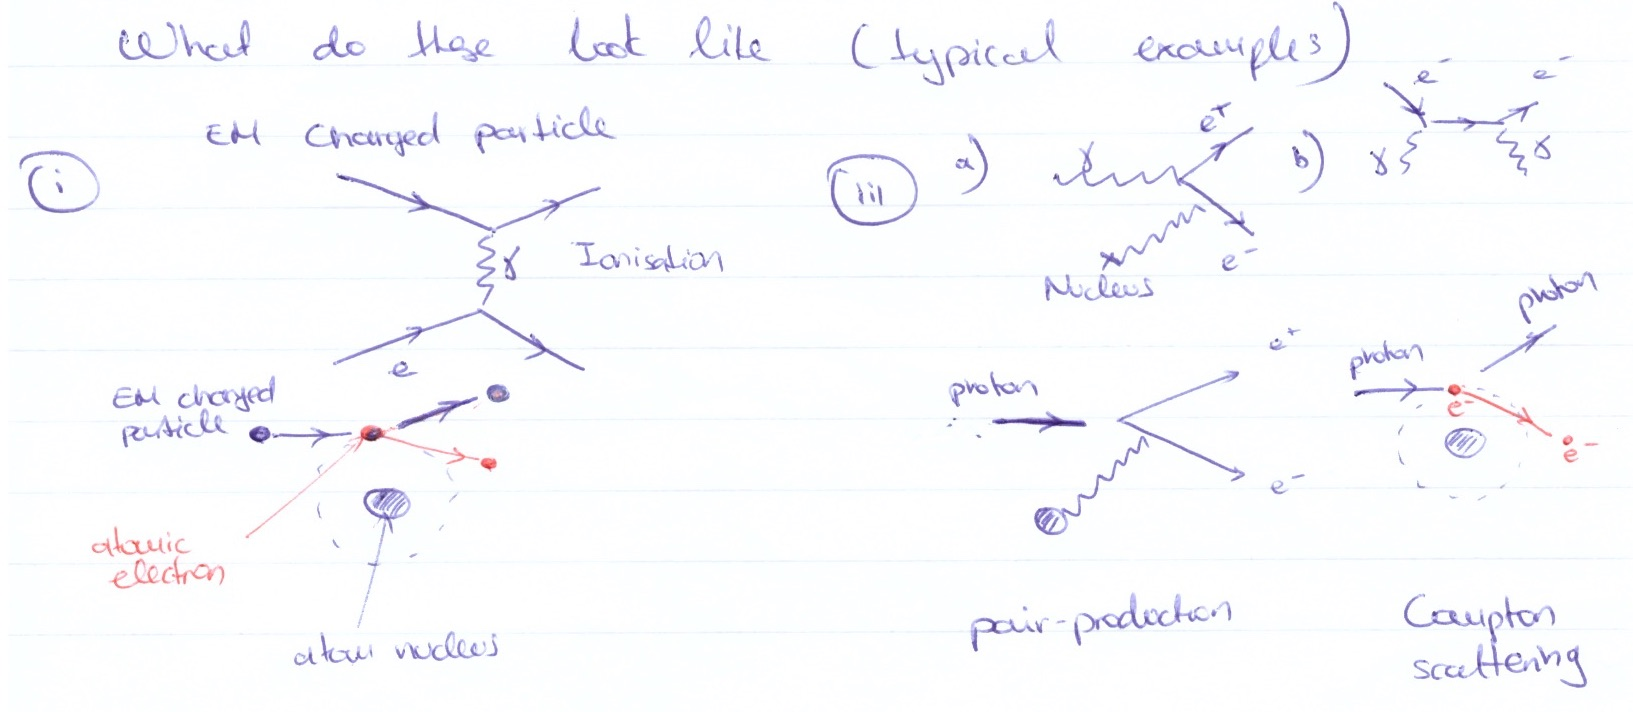
\includegraphics[width=0.95\textwidth]{fig/strongforce/matterinteractions/interactions1.jpg}\newline
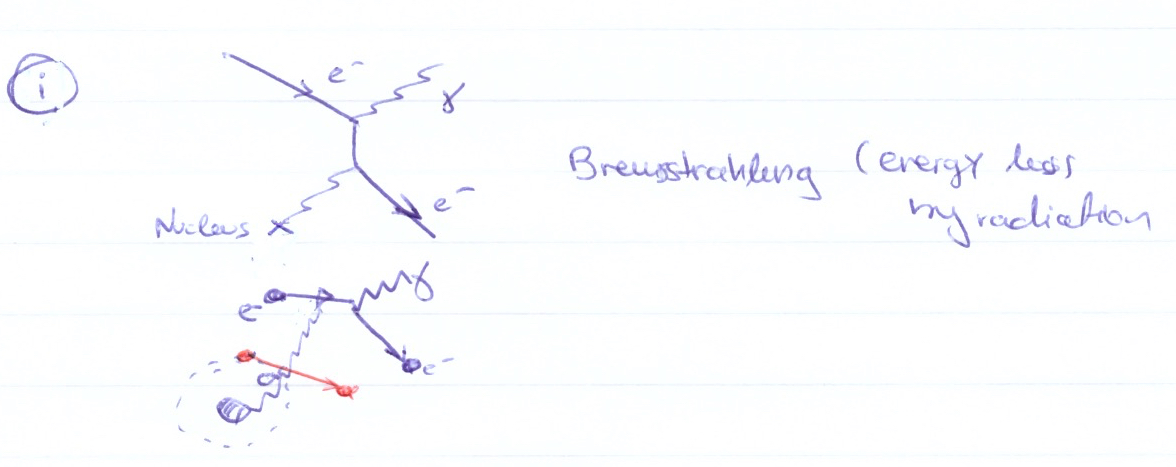
\includegraphics[width=0.8\textwidth]{fig/strongforce/matterinteractions/interactions2.jpg}
\end{center}

Most of this section will not be discussed in detail in the lecture. We still recommend you read it - it's quite interesting! But if you are in a rush, skip straight to \secref{sec:detectorSummary}.

\subsection{Energy loss through ionisation*}
We can quantify the energy loss of a particle traversing through the detector, by looking at the average rate of energy lost per unit distance.


For an incident particle of charge $ze$ with mass $M\gg m_e$, losing energy by ionising atomic electrons in a material with atomic number $Z$ we can use the Bethe-Bloch equation:

\begin{equation}
\label{eq:bethebloch}
<\frac{dE}{dx}>\approx -2C\frac{m_ec^2Zz^2}{\beta^2A}\rho\left[\frac{1}{2}\log\frac{2m_ec^2\beta^2\gamma^2T_{\rm max}}{I^2}-\beta^2-\frac{\delta(\beta\gamma)}{2}\right]
\end{equation}
with \[C=2\pi N_A\frac{e^2}{4\pi\epsilon_0m_ec^2}.\] 
$I$ is the mean ionisation potential ie $h<\nu_e>$ (given by $\sim10Z$~eV for $Z>20$), $\rho$ is the density of the material, $\delta(\beta\gamma)$ is a density correction term because the incoming particle can polarise the medium, and $T_{\rm max}$ is the maximum energy transfer in a single collision given by
\[
T_{\rm max}=\frac{2m_ec^2\beta^2\gamma^2}{[1+2\gamma m_e/M +(m_e/M)^2].}
\]
For $\frac{\gamma m_e}{M}<<1$, $T_{\rm max}$ can be simplified to
\[
T_{\rm max}\sim2\gamma^2\beta^2m_ec^2.
\]

\paragraph{Important points:}
\begin{itemize}
\item Energy loss proportional to $\frac{1}{\beta^2}$ at low speeds
\item Relativistic effects result in a slow rise at higher speeds
\item Minimum energy loss occurs (``minimum-ionising'') for $\sim (3-4)\beta\gamma$ and features largely independent of material
\end{itemize}

\subsection{Energy loss through radiation*}
Energy loss by radiation also known as ``Bremsstrahlung'' or breaking radiation occurs when a relativistic charged particle changes direction due to the influence of the field of the charged nuclei of the material. Now you should know that the change of direction, ie acceleration of a charged particle, results in the production of EM waves. In this case the energy emitted per unit length is given by
\begin{equation}
\frac{dE}{dx}\propto \frac{E}{m^2},
\end{equation}
where $m$ is the rest mass of the charged particle. This means that Bremsstrahlung energy losses are much more prominent for electrons than for pions or muons. We can write the energy lost per unit distance as
\begin{equation}
\frac{dE}{dx}=-\frac{E}{X_{0}},
\end{equation}
where $X_0$ depends on the material composition and the charge and mass of the incoming particle. We typically define $X_0$ for electrons. We therefore have that
\begin{equation}
E=E_0e^{-x/X_0},
\end{equation}
where $E_0$ is the initial energy of the electron.
It is evident that $X_0$ denotes the mean distance over which a relativistic electron loses $E_0/e$ of its energy. The CMS detector uses lead tungstate crystals (PbWO$_4$) which have $X_0=0.89$~cm.

The fact that electrons radiate a lot more energy as they are deflected (accelerated) compared to say protons, means that building circular accelerators instead of linear accelerators for electrons, has its positives and negatives. The benefit of a circular accelerator is that you can save space (and money) by being able to cycle the beam in a given ring, increasing its energy as the beam circulates many many times, without having to build a very long accelerator. However the downside is that given electrons radiate away a large amount of energy when bending in a circular orbit, you need to make sure you supply more energy each time which in turn also costs money.

Considering both loses due to ionisation and Bremsstrahlung we have
\begin{equation}
\frac{dE}{dX}(\rm total)=\frac{dE}{dX}({\rm ionisation})+\frac{dE}{dX}({\rm bremsstrahlung})
\end{equation}

For typical electron energies produced in colliders $E_{e}\sim 1-100$~GeV (ie $\gg10$~MeV), therefore Bremsstrahlung emission dominates as shown in the figure below.
\begin{center}
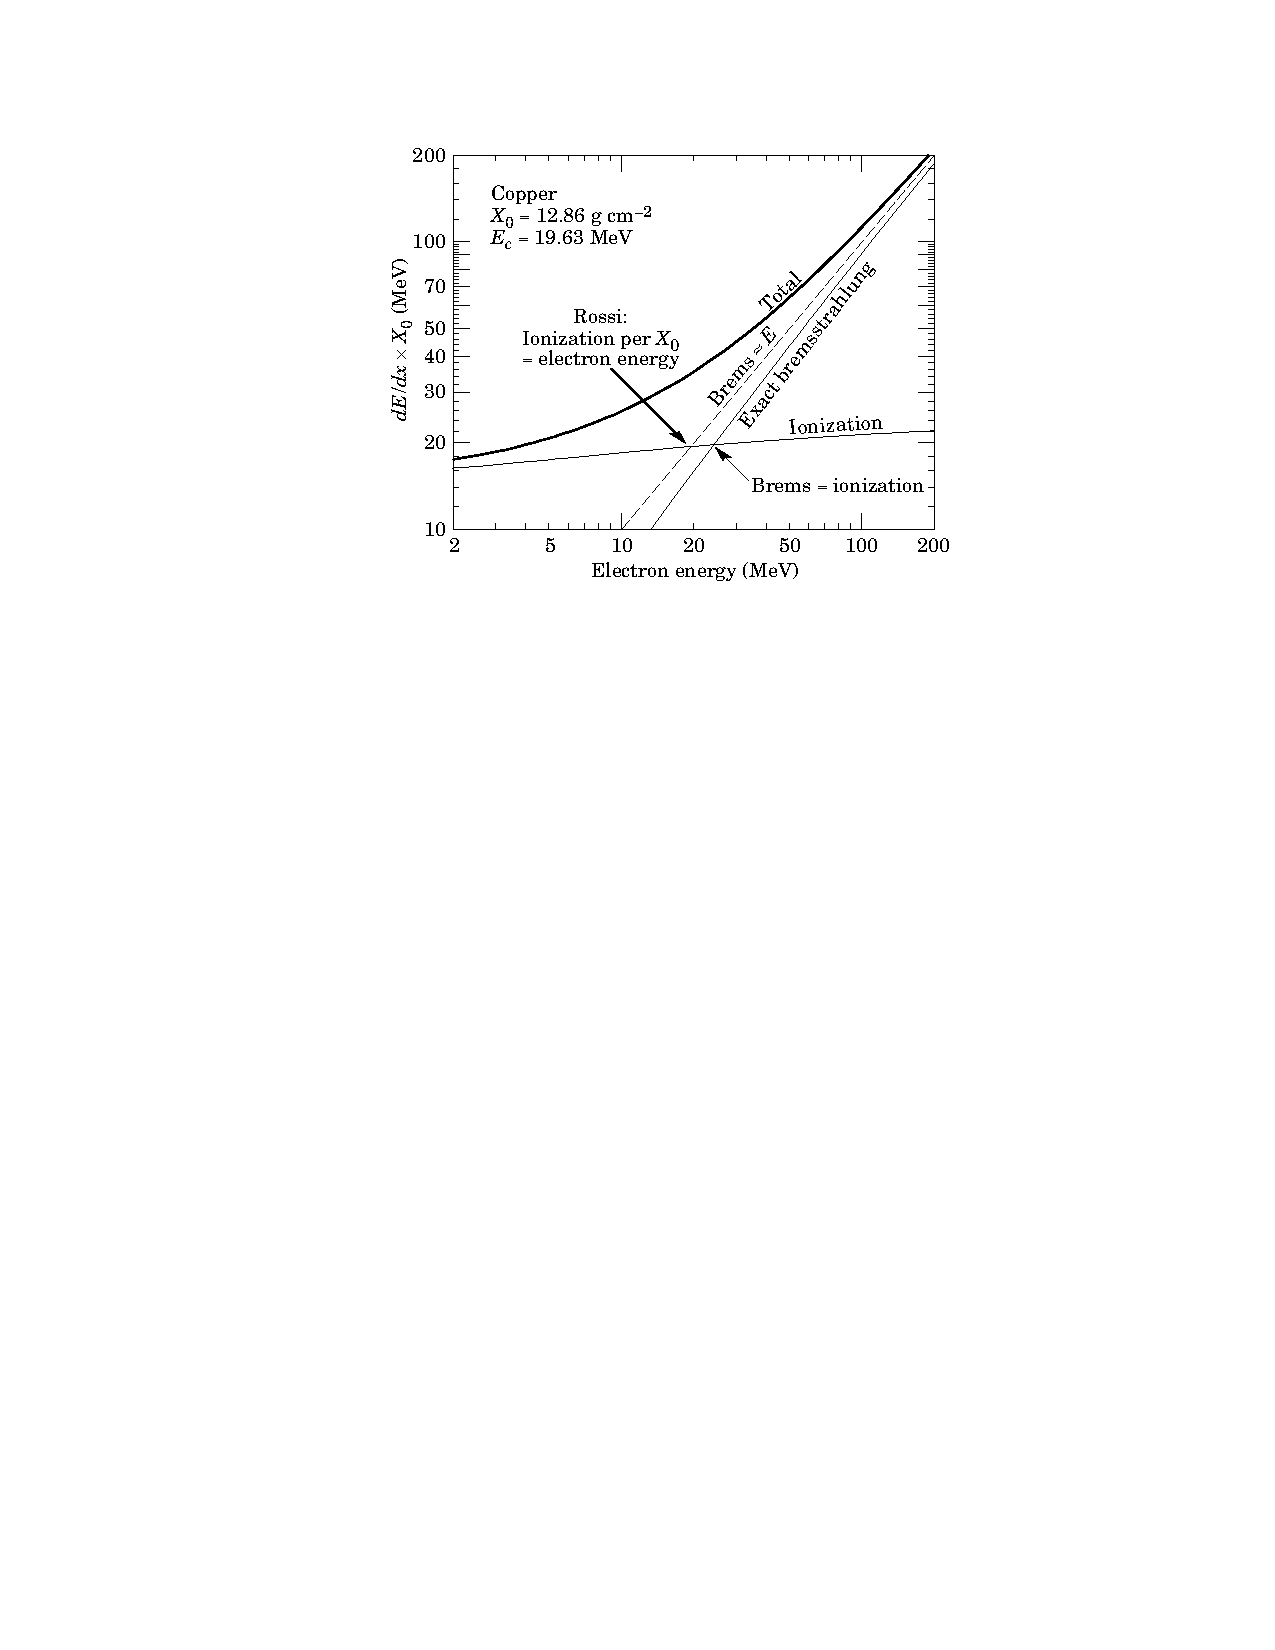
\includegraphics[width=0.6\textwidth]{fig/detector/e_energy_brem_vs_ion.pdf}
\end{center}

\subsection{Photon interactions with matter*}
Energies of photons relevant at most particle physics experiments $\gg10$~MeV.
At these energies pair production in the presence of the EM field of the charged nuclei dominate. At lower energies, Compton-scattering and the photo-electric effect dominate.
\begin{center}
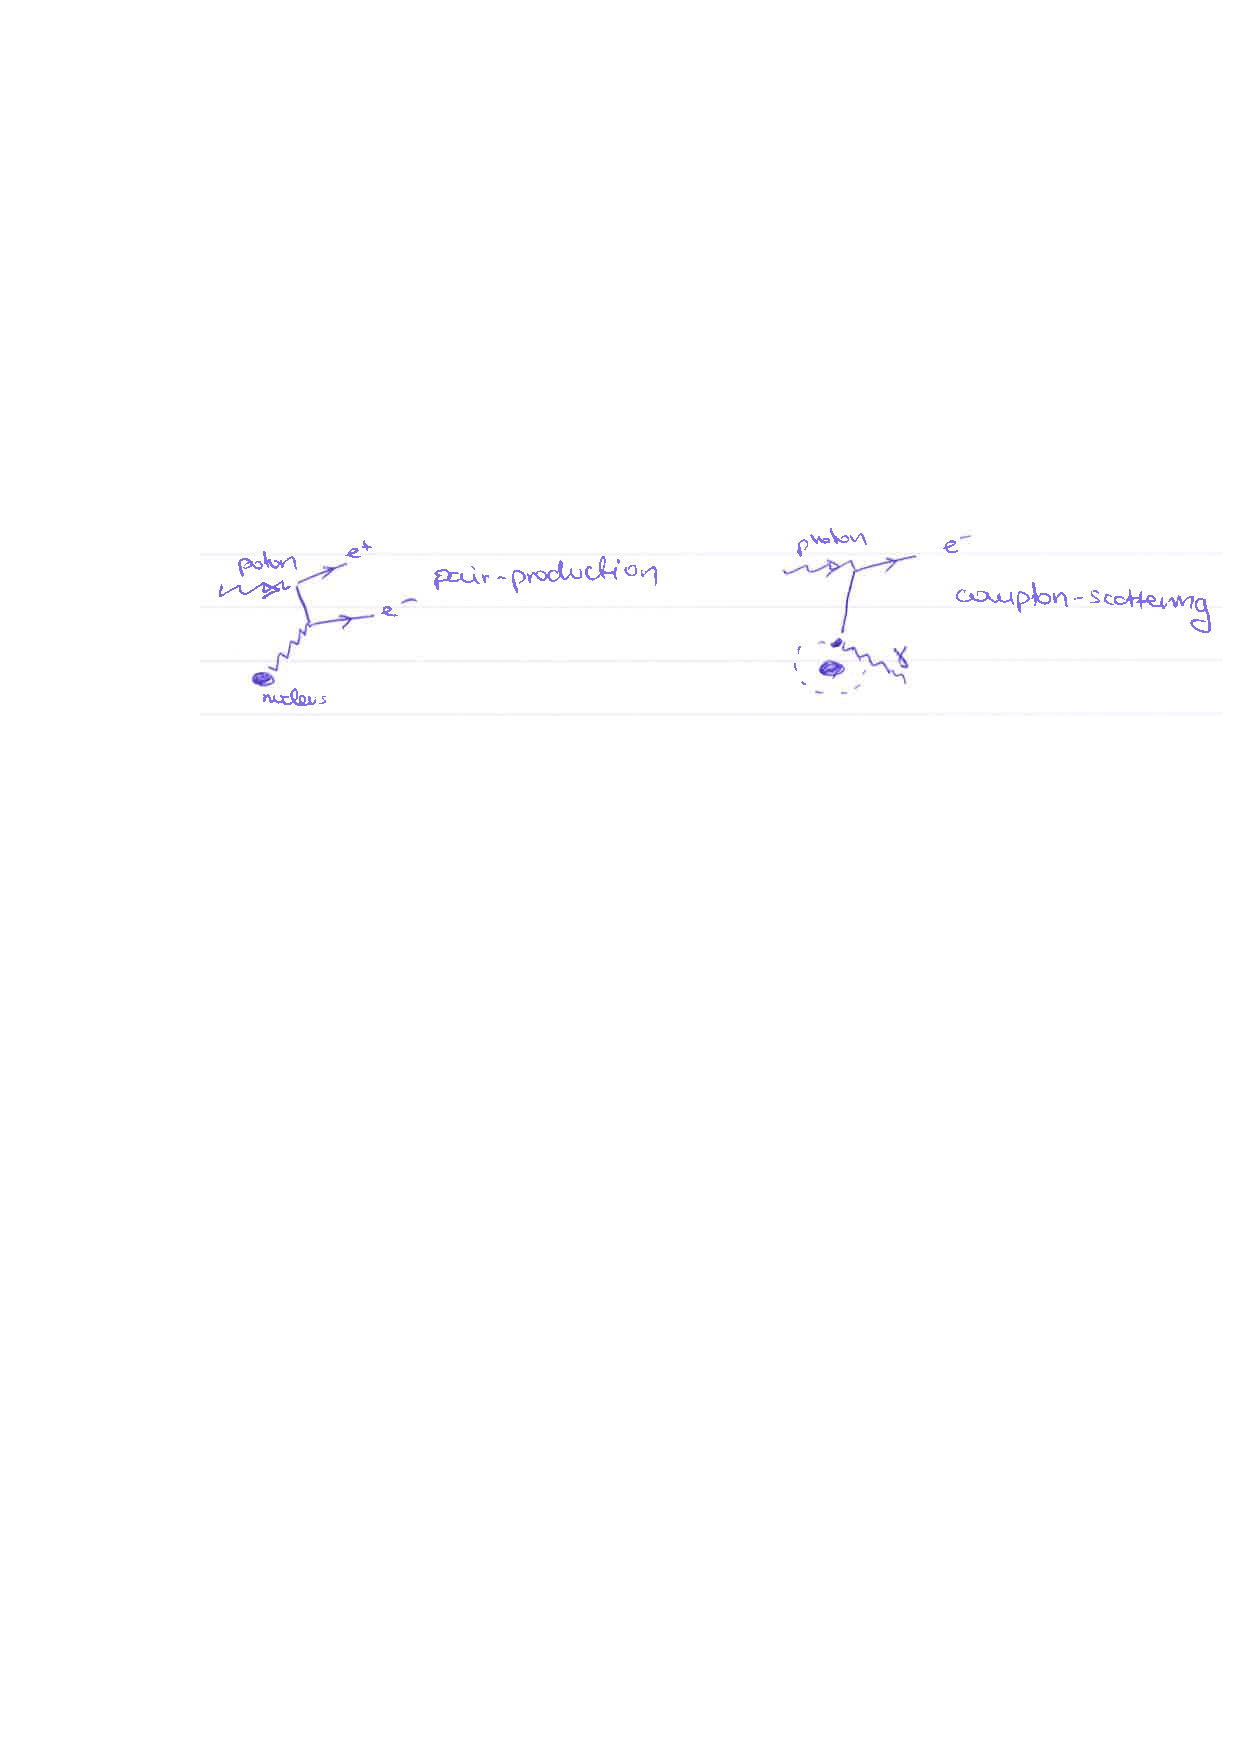
\includegraphics[width=0.95\textwidth]{fig/detector/photon_interactions.pdf}
\end{center}
Pair production has an energy threshold of $E_{\gamma}\geq 2m_{e}\sim1$~MeV. Below this energy, photons will lose energy via Compton scattering.
\begin{center}
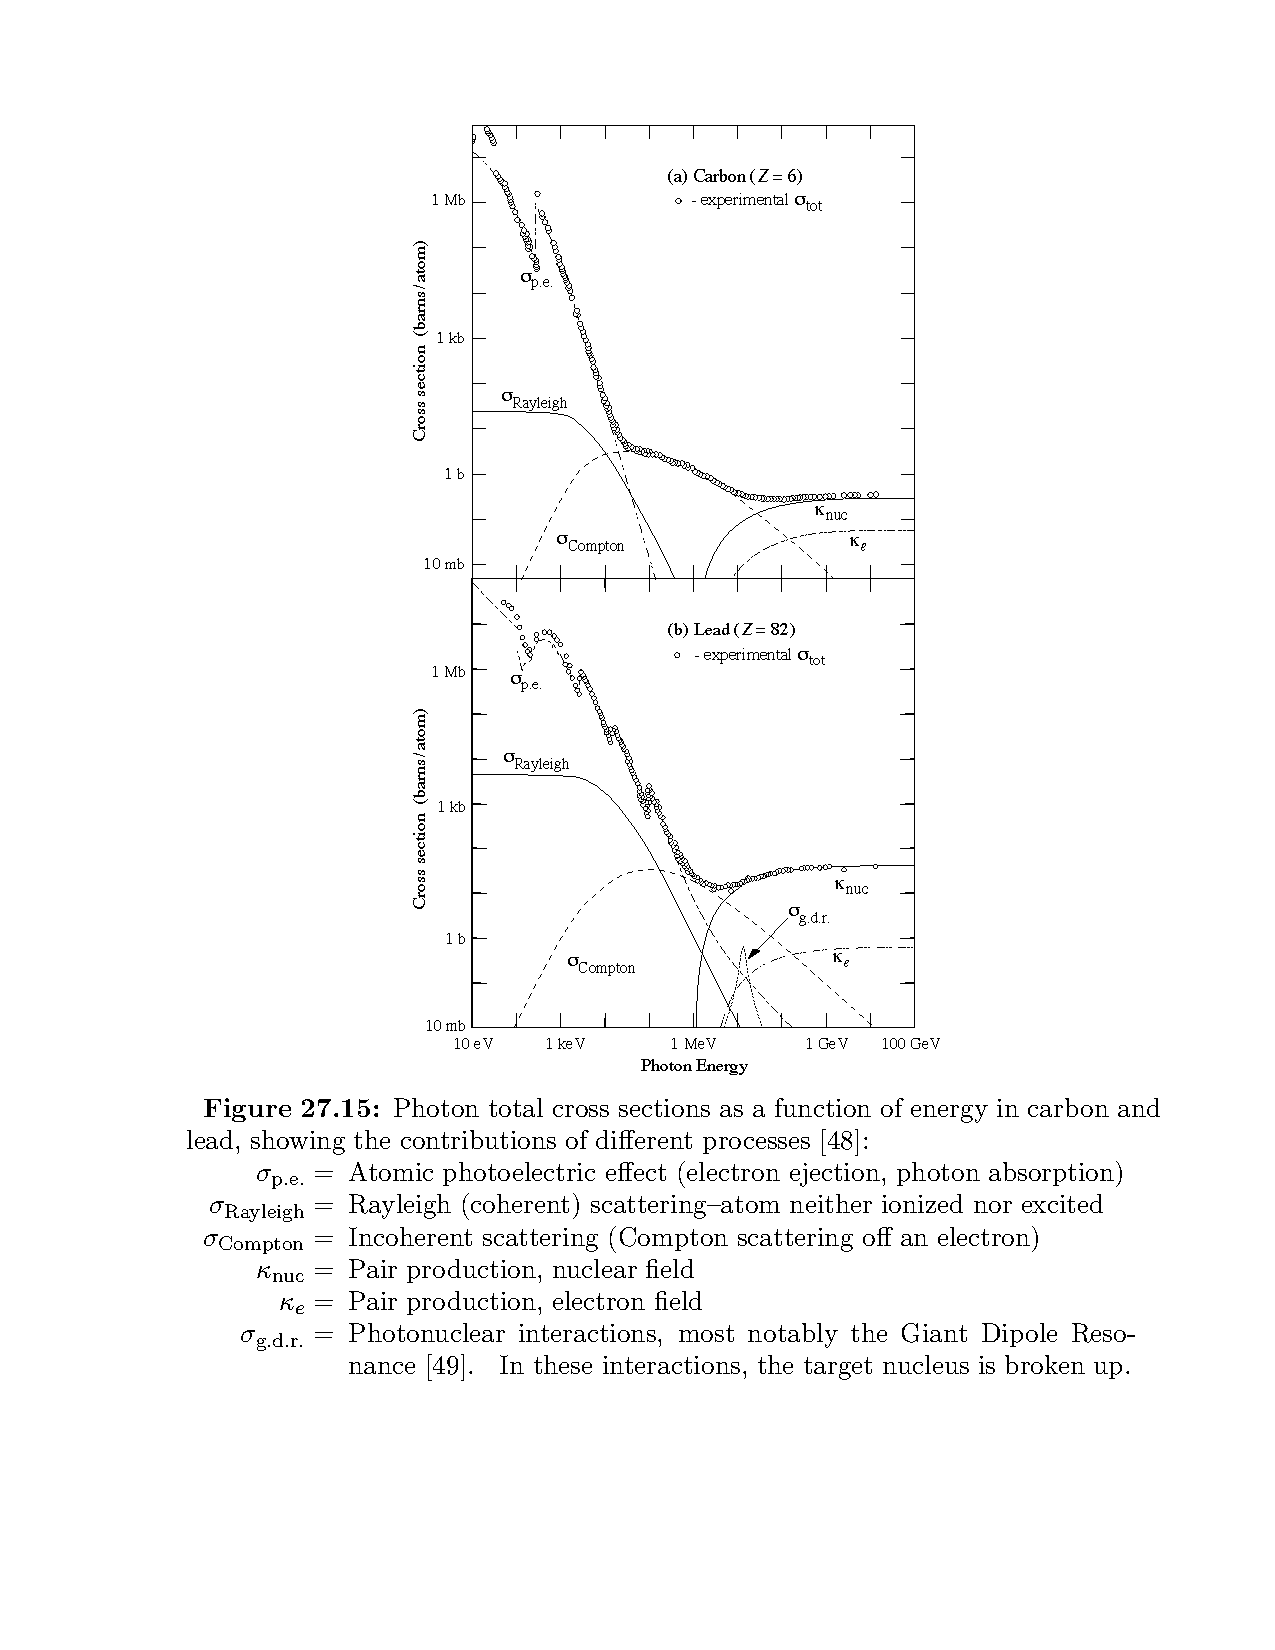
\includegraphics[width=0.90\textwidth]{fig/detector/photon_interactions_pdg.pdf}\\\tiny{Source:Particle Data Group}
\end{center}

\subsection{Electromagnetic showers*}
Incident electron or photons on thick material produce a cascade of EM processes through a chain of Bremsstrahlung and pair-production. A simplified picture is given below:
\begin{center}
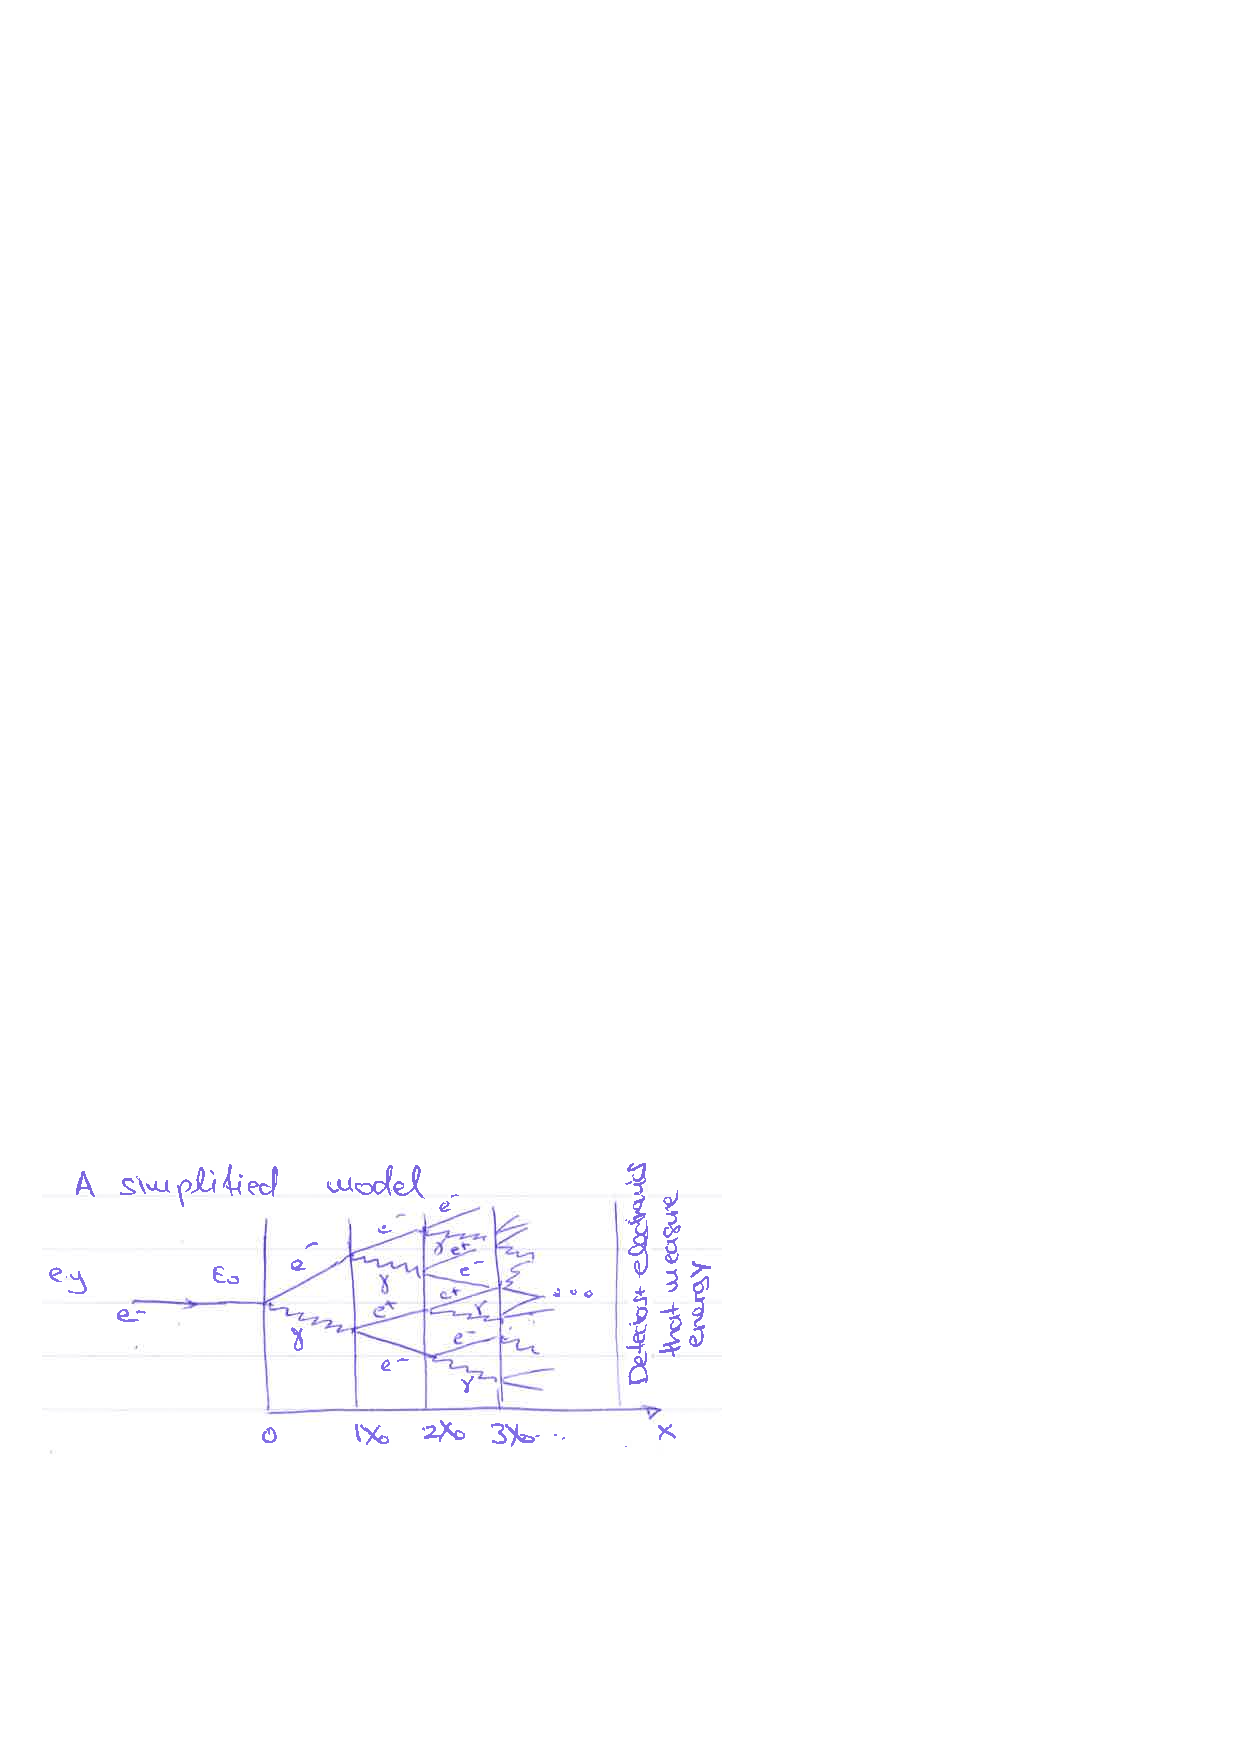
\includegraphics[width=0.90\textwidth]{fig/detector/em_shower.pdf}
\end{center}
In this simplified model, an interaction occurs every $X_0$. Assume radiation length of Bremsstrahlung and of pair-production is the same (in reality $\sim25\%$ different). 
Number of particles grows as $2^n$ where n is the integer number of radiation lengths. Energy per particle falls at each step as $E_02^{-n}$.
When electron energy falls below a critical level energy loss via ionisation dominates. Photons on the other hand loose energy via compotn scattering until the absorbed via the photoelectric effect.

Such detectors measure the energy of photons and electrons produced from the collision or from the decay of particles. These are called Electromagnetic Calorimeters (ECAL).
\subsection{Hadronic showers*}
Hadrons as as $\pi^{\pm}$, $p$, $n$ can interact with nucleons in nucleus via te strong force. So in a dense material we can have:
\[\pi^-+p\to n+\pi^0\]
ie in incoming pion on the proton of a dense material will interact via the strong force and produce a $\pi^0$ and a $n$. The $n$ will cause a subsequent strong interaction causing a hadronic shower in complete analogy to the EM shower. The $\pi^0$ will decay to a pair of photons which will initiate an EM shower. Therefore the situation with hadronic interactions with dense material is more complicated as you can get a combination of hadronic and EM showers.
In contrast to EM showers, the mean distance for a hadronic shower is called in interaction length $\lambda$ and has typical sizes of $\mathcal{O}(10)$~cm compared to interaction lenghs of $\mathcal{O}(1)$~cm. Detectors meant to measure energies of hadrons are called hadronic calorimeters (HCAL) and due to the larger showers, they tend to be larger than ECALs.

\subsection{Cherenkov radiation*}
A charged particle that moves in a medium with a velocity larger than the velocity of the speed of light in this medium (ie $v>c/n$ where $n$ is the refractive index of the medium), will emit a cone of light very much like the cone of sound of a sonic boom of an aircraft breaking the sound barrier (or like the ripples a duck produces as it swims in the pond)
\begin{center}
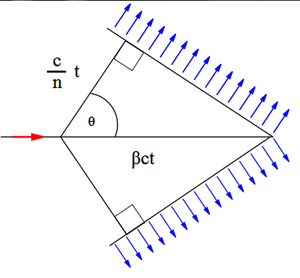
\includegraphics[width=0.45\textwidth]{fig/detector/cherenkov_angle.png}
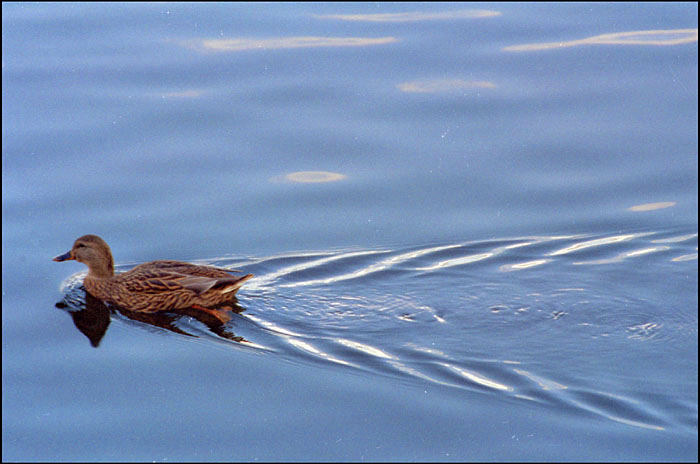
\includegraphics[width=0.45\textwidth]{fig/detector/duck_angle.png}
\end{center}
So photons are emitted at an angle $\theta_c$ given by 
\begin{equation}
\label{eq:cherenkov_angle}
\cos\theta_{C}=\frac{1}{n\beta}
\end{equation}
By placing a gas or liquid volume in path of the particle and surround this volume by photon detectors, the resulting Cherenkov photons form a ring. We call these detectors Ring Imaging Cherenkov (RICH) detectors. 
\begin{center}
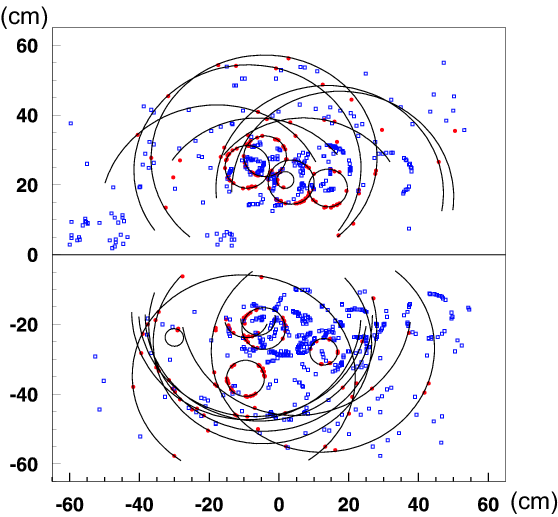
\includegraphics[width=0.75\textwidth]{fig/detector/rich_1_rings.png}
\end{center}
Measuring the Cherenkov angle allows to determine the speed of the particle. Combined with a measurement of the momentum of the particle, we can therefore determine very accurately the mass and hence the type of particle. An important point to remember and which also stems from Eq.~\ref{eq:cherenkov_angle}, is that Cherenkov radiation is only emitted if $\beta>\frac{1}{n}$. Additionally, as the particle's speed increases, $cos\theta_{C}$ approaches $\frac{c}{n}$ asymptotically. Thus the ability to determine the speed of the particle becomes more and more difficult as the ring size changes less and less. A solution is to have two RICH detectors with materials of different $n$, in order to have good resolution for a large range of particle speeds.
\begin{center}
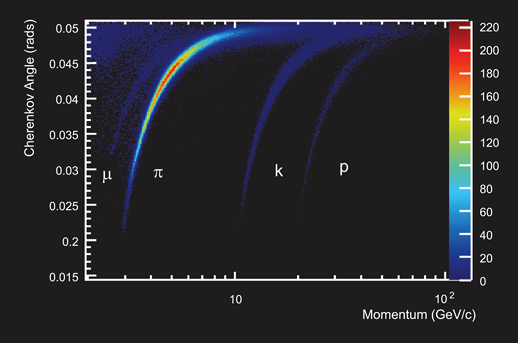
\includegraphics[width=0.75\textwidth]{fig/detector/lhcb_cherenkov_vs_momentum.png}
\end{center}

\subsection{Putting it all together}
\label{sec:detectorSummary}
\begin{center}
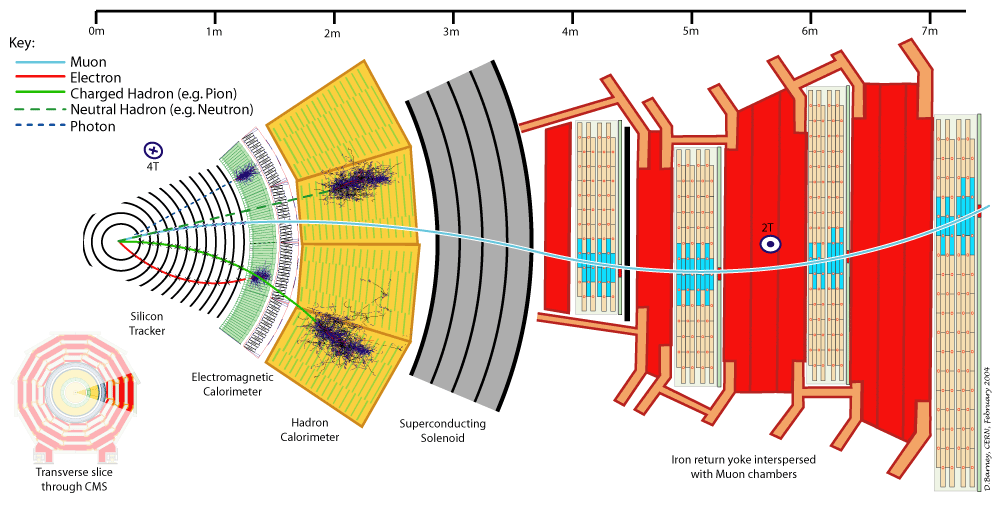
\includegraphics[width=0.95\textwidth]{fig/detector/cms_slice.png}
\end{center}

The inner most part of a detector is typically made up of relatively low radiation and interaction length material aimed at making a precise measurement of the initial collision point and of subsequent decay vertices. This is achieved by reconstructing the trajectories of outcoming charged particles as they deposit energy via ionisation. They are called ``vertex detectors'' and are typically made up of silicon pixel or strip sensors. 

Following the vertex detectors, one finds further detectors aimed at reconstructing the trajectories of charged particles by detecting ionisation energy as the particles traverse through them (``Tracking detectors''). By placing a magnetic field and measuring how the trajectory of the particles bends, we can get an estimate of their momentum.

Past the tracking detectors one can place RICH detectors (e.g at LHCb) aimed at measuring the speed of the particle, and combining with the measurement of the momentum obtain an estimate of the particle's mass and hence its type. One can also place an ECAL after the tracking (and after the RICH systems) to measure the energies of photons and electrons. As hadrons have masses much larger than the electron mass, they will not have an EM shower in the ECAL and will not form a hadronic shower either, as the typical interaction length ($\lambda$) of the ECAL is much too small (ECALs are less dense than HCALs). 

After the ECAL follows the HCAL. In the HCAL hadrons like pions, Kaons and protons will perform a hadronic shower, allowing for the measurement of their energies. Energies of jets of hadrons initiated by quarks and gluons, are measured by combining information from the tracking systems and calorimeters.

Muons are a special case. As $m_\mu\sim m_\pi\gg m_e$ and muons do not undergo strong interactions, they pass through the ECAL and HCAL by simply depositing a minimum amount of ionisation energy. Therefore in order to detect muons, detection systems aimed at measuring deposits of ionisation energy are placed after the HCAL, allowing for both the identification of muons (as mainly muons would reach the outer parts of the detectors) as well as the measurement of the momentum as the muon bends in the magnetic field. Muons are therefore very easy to distinguish from other particles: They are the one charged particle that makes it through all the mass in the calorimeters and survives until the muon detectors. Particle physicists love decays with muons int he final state!

\begin{center}
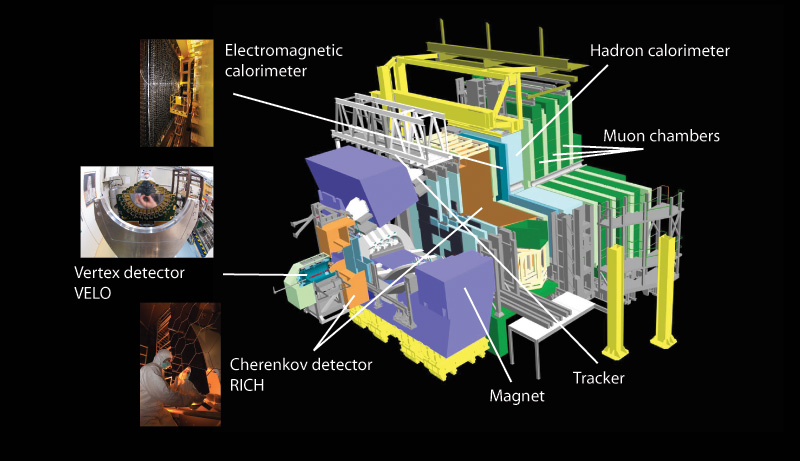
\includegraphics[width=0.95\textwidth]{fig/detector/lhcb_detector.png}
\end{center}
The figure below shows a similar configuration for the LHCb detector.

\subsection{Missing transverse momentum (or energy)}
This has already been discussed in \secref{sec:missingEt}, but is repeated here under a slightly different angle, because it also belongs into the detector section, and because it is important.

In hermetic ($4\pi$) detectors like CMS and ATLAS, particles that only very rarely interact
with matter (such as neutrinos and particles proposed in theories beyond the Standard Model such as Supersymmetry or hypothesised Dark Matter candidate particles) are detected by their absence. What do we mean by that? 

In a $pp$ collision (or any collision) where the protons are primarily only have momentum along the horizontal axis, the total initial momentum transverse to the direction of the protons is zero. Therefore after the collision, momentum should be conserved and thus the total momentum obtained by summing over all the outcoming particles from the collision (this is why detectors like CMS that completely surround the collision are important), transverse to the direction of the protons ie 
\[{\rm Missing\,\,Transverse\,\,Momentum}=-\sum_{\rm i=1..N_{\rm particles}} p_{T}^{i}\]
should add up to zero. If it does not then it means that particles where produced which did not interact with the detector. Such particles could have been known neutrinos or, depending on the amount of missing energy, momentum could be Dark Matter candidates.
The figure below, is a $t\bar{t}$ event from CMS where each of the $t$-quarks decay to a $b$ quark (which forms a jet) and a $W$ boson which subsequently decays to a $\mu$ and a $\nu_{\mu}$. The sum of the momenta that the two $\nu$'s carry (one from the $t$ and another from the $\bar{t}$) is inferred by the mis-balance of momentum (or equivalently energy) in the transverse plane and is denoted by the purple arrow labelled $\cancel{\rm E_{T}}$.
\begin{center}
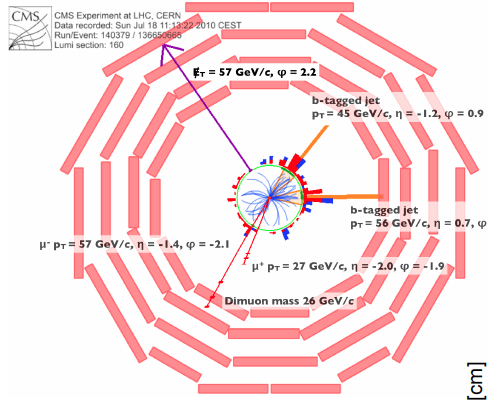
\includegraphics[width=0.75\textwidth]{fig/detector/met_cms.png}
\end{center}

An example of a process that makes use of all detector components of the detector is the production of top quarks at the LHC. Top quarks have a very short lifetime. 
\[\tau_{t}=5\times 10^{-25}s\]
However the time at which QCD confinement acts (ie the time scale in which a quark binds into a hadron) can be calculated as follows:

QCD confinement takes place at an energy scale 
\[
\Lambda_{QCD}=200~{\rm MeV}.
\]
We can convert this energy scale into a timescale using 
\[
\hbar c=200~{\rm MeV~fm}
\]
(this is something you should commit to memory as it is a very useful quantity for a particle physicist).
Therefore
\[
\tau_{QCD}=\hbar c\times\frac{1}{c\Lambda_{QCD}}=3\times 10^{-24}s
\]
As $\tau_{QCD}<\tau_{t}$, the top quark decays before it has a change to form a bound state! 

Due to the CKM elements involved, the top quark predominantly decays to a b-quark 
\[t\rightarrow b W\]
where the $b$-quark will in turn produce a jet of particles which contains at least one hadron with a $b$-quark. This so called $b$-jet can be identified both through the stream of hadrons producing tracks in the tracking system and energy depositions in the calorimeters, as well as through the displaced vertex formed by the decay products of the $B$-hadron.
The $W$ will in turn decay into a lepton or a pair of quarks. In the case that the $W$ decays to a lepton and a neutrino, the neutrino escapes the detector and its existence is inferred through missing transverse energy.